\documentclass[aps,letterpaper,11pt]{article}

\usepackage{graphicx} % For images
\usepackage{float}    % For tables and other floats
\usepackage{verbatim} % For comments and other
\usepackage{amsmath}  % For math
\usepackage{amssymb}  % For more math
\usepackage{fullpage} % Set margins and place page numbers at bottom center
\usepackage{listings} % For source code
\usepackage{subfig}   % For subfigures
\usepackage[usenames,dvipsnames]{color} % For colors and names
\usepackage[pdftex]{hyperref}           % For hyperlinks and indexing the PDF
\usepackage{libertine}
\usepackage[T1]{fontenc}
\usepackage[scaled]{beramono}
%\usepackage{lmodern}
%\usepackage{tgadventor}
\usepackage{multicol}
\usepackage[usenames,dvipsnames]{color}
\hypersetup{ % play with the different link colors here
     colorlinks,
      }
\begin{document}


% title page/cover
\begin{titlepage}
\begin{center}

{\Huge 
Uplink User-Assisted Relaying \\ in Cellular Networks 
}~\\[4cm]

% The '~' is needed because \\ only works if a paragraph has started.

{\large 
Dual Degree Project 1st Stage Report
}~\\[2cm]

\end{center}

\begin{multicols}{2}
\begin{flushleft}
{\large
\textit{Student:} \\
\text{Prudhvi Porandla} \\
\text{Roll No: 110070039}
}
\end{flushleft}
\columnbreak
\begin{flushright}
{\large
\textit{Guide:} \\
\text{Prof. S. N. Merchant}
}
\end{flushright}
\end{multicols}

\vfill

\begin{center}

\includegraphics[width=4cm]{figures/iitbblack.jpg}~\\[1cm]

{\large
Department of Electrical Engineering\\
Indian Institute of Technology Bombay\\
Mumbai 400076, India\\
}

\end{center}
\end{titlepage}
% cover page end
\pagenumbering{roman}

\mbox{}
\newpage

\tableofcontents
\newpage
\mbox{}
\newpage
~\\[6cm]
\begin{abstract}
Currently, there are 31,254 level crossings and around 40\% of them are unmanned. The unmanned
crossings are responsible for the maximum number of train accidents. The m
ain objective of this project
is to reduce the number of such accidents by building a reliable system th
at can consistently detect a train
moving towards the crossing and sets off an alarm at the crossing.
\end{abstract}
\newpage
\mbox{}
\newpage


\section{Introduction}
The solution to this problem is to build a system that can turn on an alarm at the crossing at least 1 min
before the train reaches the crossing and turn off the alarm when the train passes the crossing. To do this, we
designed a sensor unit, using two inductive proximity sensors, that can detect a train and its direction,
and an alarm unit. The sensor unit will be placed 1.5 km away from the crossing while the alarm unit will be
placed at the crossing. When a train passes over the two sensors of the sensor unit, it detects the direction
of the train, counts the number of axles\footnotemark\footnotetext{We actually count the number of wheels on one side, 4 wheels on each side $\implies$ 4 axles}($n$) and sends this information to the alarm unit. If the train is moving
towards the crossing, alarm unit turns on the alarm. When the train passes over the single sensor placed at the crossing,
the alarm unit down counts the number of axles from $n$ and turns off the alarm when the count reaches 0.
\\ \\
In the next sections we present the block and circuit diagrams of various units of the system, different
algorithms used to detect the direction of train and also how false alarm cases are handled.
\pagenumbering{arabic}

\section{Block Diagrams}
\subsection{Functional Block Diagram}

\begin{figure}[H]
\begin{center}
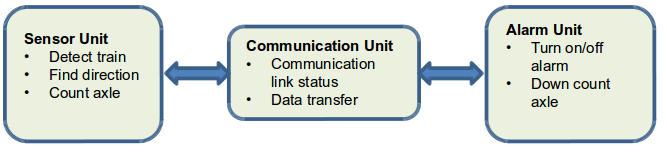
\includegraphics[height = 1.5in,width=5.5in,angle=00]{figures/block1.png}
\caption{\small This figure shows overall working of the system}
\end{center}
\end{figure}
\subsection{Communication unit}
Functions:
\begin{enumerate}
  \item Check if communication link is active
  \item Data transfer
\end{enumerate}

\begin{figure}[H]
\begin{center}
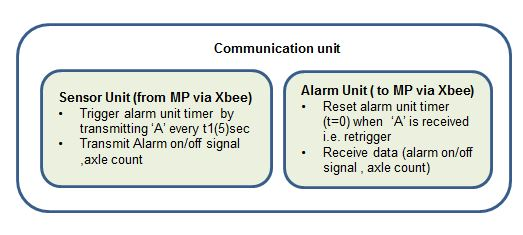
\includegraphics[height = 1.65in,width=4.5in,angle=00]{figures/block3.JPG}
\caption{\small Communication unit}
\end{center}
\end{figure}
\subsubsection{Link check}
We are using a watchdog timer at the alarm unit to check if the communication
link
between sensor unit and alarm unit is active.
\begin{figure}[H]
\begin{center}
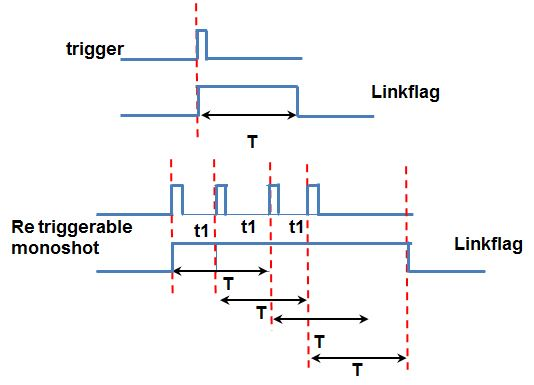
\includegraphics[height = 2in,width=4in,angle=00]{figures/block2.JPG}
\caption{\small Watchdog timer at alarm unit}
\end{center}
\end{figure}
\begin{itemize}
\item Sensor unit triggers by sending some packet (char `A') to alarm unit,
when alarm unit
receives this packet it initializes timer (t=0), when timer = T (t=T) it
resets \texttt{Linkflag}
(\texttt{Linkflag}=0).
\item Sensor unit will trigger every t1 sec and alarm unit initializes timer
to zero (t=0) setting
the \texttt{Linkflag} high (\texttt{Linkflag}=1). In this process \texttt{
Linkflag} stays high (\texttt{Linkflag}=1) as long
as the communication link is active.
\item \texttt{Linkflag} is low (\texttt{Linkflag}=0) implies that it did not
receive any packet for the last T sec and the link in not active.
\end{itemize}
\subsubsection{Data Transfer}
In our application only sensor unit transmits and alarm unit receives. Sensor
unit transmits the
following signals.
\begin{itemize}
\item Alarm on signal `D' when train is detected
\item Axle count `W'
\item Sensor unit active signal `A'
\item False alarm signal `F' in case of false alarm
\end{itemize}
\subsection{Sensor unit}
Functions:
\begin{itemize}
  \item Detect direction of train in case of bidirectional track
  \item Send alarm on signal `D'
  \item Send axle count to alarm unit `W'
  \item Send sensor unit active signal `A'
  \item Detect false alarm and turn off alarm
  \item Send its device ID every time some packet is sent
\end{itemize}

We will discuss above functionalities, and how we take care of errors in
each of the following cases:
\begin{itemize}
  \item Unidirectional track
  \item Bidirectional track
  \item Multiple unidirectional tracks
\end{itemize}

The following assumptions are made:
\begin{itemize}
  \item Alarm gets info about the train at least 1 min before it arrives at the crossing
  \item The average maximum speed of the train is 90 kmph.
  \item The train's acceleration doesn't have significant effect on the arrival time.
   Above two assumptions imply that the sensor unit (s1, s2) should be placed 1.5 km away from crossing and s3 at 100 m from the crossing on the other side.
  \item The distance between the sensors s1, s2 must be $p$ \footnote{$p$ < distance between wheels} m.
\end{itemize}

\subsubsection{Unidirectional track}
On this track, trains move only in one direction (left to right in Figure 4)
\begin{figure}[H]
\begin{center}
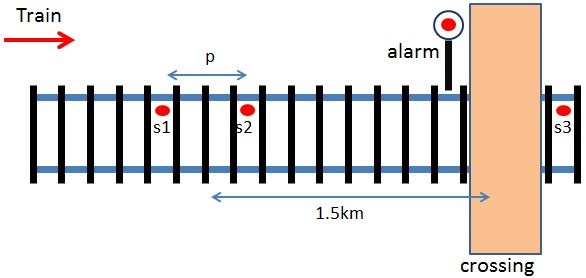
\includegraphics[height = 2in,width=4in,angle=00]{figures/oneWayTrack.JPG}
\caption{\small Unidirectional track}
\end{center}
\end{figure}
When train crosses sensor unit the following pulse pattern occurs on sensors (
s1, s2).

\begin{itemize}
\item Case 1: No pulse is missed \\
\begin{figure}[H]
\begin{center}
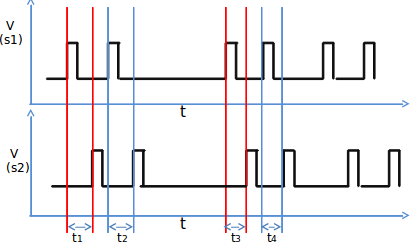
\includegraphics[height = 2in,width=4in,angle=00]{figures/8w_no_miss.png}
\caption{\small pulses on s1, s2 as train crosses the sensor unit}
\end{center}
\end{figure}

We start timer at the rising edge of s1 and stop the timer at rising edge of
s2. We store the time periods t1, t2, t3 \ldots{} and check if $\frac{t1}{t2}
= \frac{t2}{t3} \ldots = 1 $. We count axles only when new non zero timervalue
is recorded. When the count reaches three, it checks the ratios condition and
if this condition is true, it sends ON signal (`D') to the alarm unit. \\
The unit keeps counting the pulses and if at any moment it doesn't receive any
new pulse for 5 sec it assumes the train has crossed the sensor unit and sends
axle count to the alarm unit `W'.

\item Case 2: s2 misses some pulses \\
As the distance between two sensors is less than the distance between the
wheels we can see from Figure 5 that every rising edge of s2 lies between two
rising edges of the s1. As the timer resets at the rising edge of the s1 and
stops at the rising edge of s2, if the $1^{st}$ pulse form s2 is missed, it
won't give any wrong time because the $2^{nd}$ pulse from s1 resets timer
before arrival of $2^{nd}$ pulse of s2.
Axle count is not incremented.

\item Case 3: s1 misses some pulses \\
As the rising edge of s2 stops timer, the timer won't be reset until an s1
pulse is received. So we won't get any wrong time.
\end{itemize}

\subsubsection{Bidirectional track}
On this track, trains move in either direction.\\
Working remains same as above but the main task here is to find the direction
in which train is moving. If train is going towards the crossing, then it
should send ON signal to the alarm unit. For the alarm unit to distinguish
between the data sent by two units, the data from left unit will
have `L' and that from right unit will have `R' as the first byte.
\begin{figure}[H]
\begin{center}
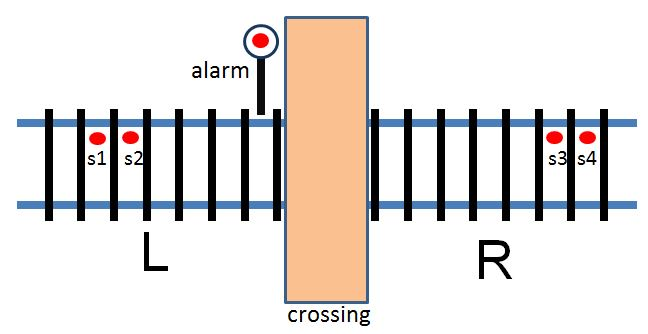
\includegraphics[height = 2in,width=4in,angle=00]{figures/twoSideSensors.JPG}
\caption{\small Sensors on a bidirectional track}
\end{center}
\end{figure}
\newpage
\subsubsection{Finding direction}
There are two types of wagons\footnote{a coach or a goods carriage}:
\begin{itemize}
\item 8 wheel/4 axle wagons (8w)
\item 4 wheel/2 axle wagons (4w)
\end{itemize}
\begin{figure}[H]
\begin{center}
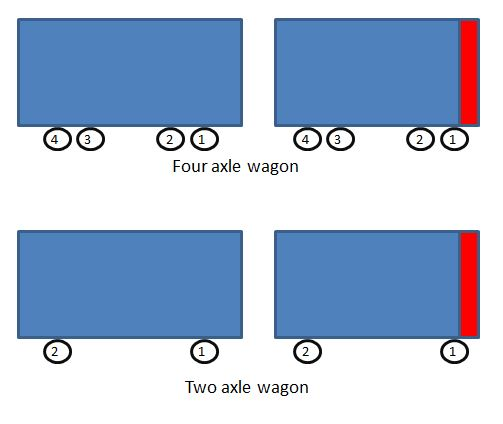
\includegraphics[height = 2.5in,width=3in,angle=00]{figures/wagonTypes.JPG}
\caption{\small 2 types of wagons; 4 axle wagons are more common}
\end{center}
\end{figure}
\underline{Four axle wagon:}
\begin{itemize}
\item Distance between 1(rightmost) \& 2 = Distance between 3 \& 4 = 2 m
\item Distance between 2 \& 3 is $l1$ = 16 m (14 m < $l1$ <18 m)
\item Distance between 4 \& 1(distance between two wagons) is $l2$ (4 m < $l2$
< 6 m)
\end{itemize}
\underline{Two axle wagon:}
\begin{itemize}
\item Distance between wheels 1 \& 2 is $l3$ (14 m < $l3$ < 18 m)
\item Distance between wheels 2 \& 1 (distance between wagons) is $l4$ (4 m <
$l4$ < 6 m)
\end{itemize}
\newpage
Consider the sensors unit to the left of the crossing (Figure 6). \\
\begin{center}
========\textbf{(s1) (s2)}======|-|=======(s3) (s4)======
\end{center}

When an 8w wagon goes from left to right, (s1) and (s2) will generate the
 following pulses
\begin{figure}[H]
\begin{center}
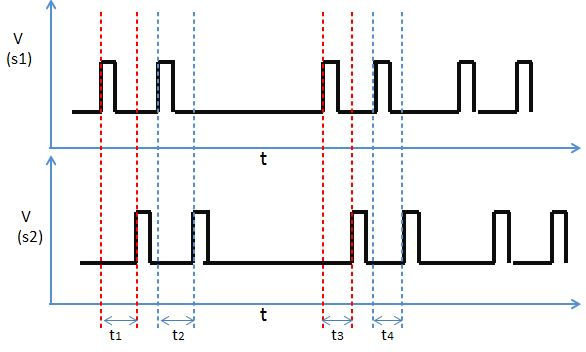
\includegraphics[height = 2in,width=4in,angle=00]{figures/w8_no_missing.JPG}
\caption{\small Pulses generated by s1, s2}
\end{center}
\end{figure}

The setting and resetting of the timer is done as follows: \\
If sx (x=1 or 2) gives the first pulse, then the pulses from that sensor will
trigger the timer reset (reset and initialize) and the pulses from the other
sensor stop the timer. In the above case rising edge of s1 resets and rising
edge of s2 stops the timer. \\
$t1$ is the time taken by the first pair of wheels to travel a distance $p$ (
separation between s1 and s2). For a train moving at constant speed, $t1 = t2
= t3 = t4 = p/v$ where $v$ is speed of the train. \\ \\
Similarly a 4w wagon going from left to right generates the pulses of the
following form:
\begin{figure}[H]
\begin{center}
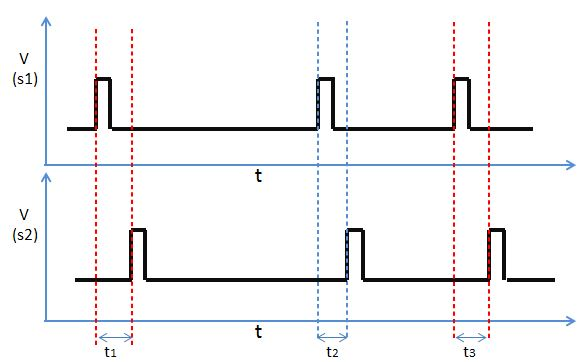
\includegraphics[height = 2in,width=4in,angle=00]{figures/w4_no_missing.JPG}
\caption{\small 2 axle wagon case, pulses on s1, s2}
\end{center}
\end{figure}

A pulse from s1 resets the timer and a pulse from s2 stops the timer. $t1, t2
$ and $t3$  are stored. $t1$ is
the time taken by the first pair of wheels to travel a distance $p$(separation
between s1 and s2). \\ \\
For a train moving at constant speed, $t1 = t2 = t3 = p/v$ where $v$ is speed
of the train. \\ \\
By this we find that no pulse is missing and we get the direction by seeing on
which sensor we got the first pulse i.e. if first pulse, from the sensor unit
to the left of crossing, is on s1 we know that train is moving from left to
right. What happens if this first pulse is missed? \\

\textbf{Case 1:} s1 misses the first pulse \\
If s1 misses the first pulse, initially we take the direction of the train as
right to left as the first pulse appeared on s2. s2 resets and s1 stops the
timer.
\begin{figure}[H]
\begin{center}
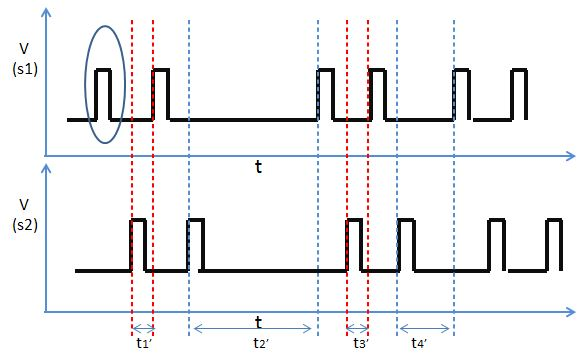
\includegraphics[height = 2in,width=4in,angle=00]{figures/w8_pulse_missing.JPG}
\caption{\small s1 misses the first pulse in 8w case}
\end{center}
\end{figure}

But now we have three different times recorded $t_1', t_2', t_4'$.
\begin{center}
$
t_1' = t_3' =\frac{2-p}{v} \qquad
t_2' = \frac{l_1-p}{v} \qquad
t_4' = \frac{l_2-p}{v}
$
\end{center}
Substituting the values of $l_1, l_2$ and taking the ratios of subsequent time
intervals
\begin{center}
$
\frac{t_2'}{t_1'} = \frac{l_1-p}{2-p} > 2 \qquad
\frac{t_3'}{t_2'} = \frac{2-p}{l_2-p} < 0.5 \qquad \frac{t_4'}{t_3'} = \frac{l_2-p}{2-p} > 2 $
\end{center}
%\newpage
\mbox{}
Similarly for a 4w wagon
\begin{figure}[H]
\begin{center}
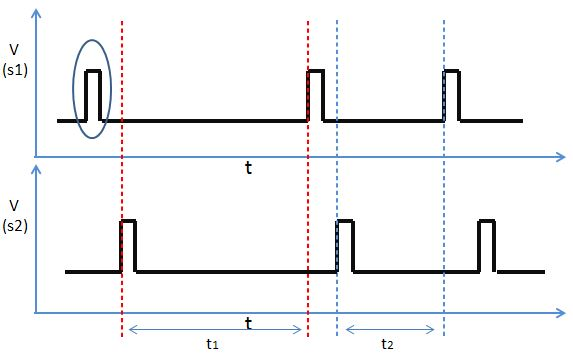
\includegraphics[height = 2in,width=4in,angle=00]{figures/w4_1_pulse_missing.JPG}
\caption{\small s1 misses the first pulse in 4w case}
\end{center}
\end{figure}
\begin{center}$\frac{t_2}{t_1} = \frac{l_3-p}{l_4-p} > 2 $ \end{center}
Whenever a pulse is missed, the ratio of subsequent time intervals, in both 8w and 4w cases, is greater than 2 or less than 0.5. Therefore by checking the ratios, we will know if the assumed direction is correct or not. If the assumed direction turned out to be wrong after the above test, the roles of pulses from s1, s2 will be reversed i.e. pulses from s1 reset the timer and pulses from s2 stop the timer or viceversa \\ \\

\textbf{Case 2:} s2 misses its first pulse \\
\begin{figure}[H]
\begin{center}
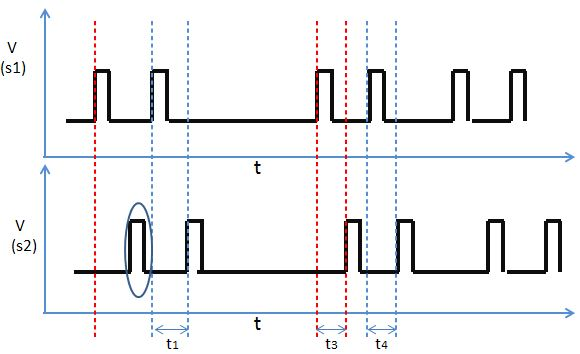
\includegraphics[height = 2in,width=4in,angle=00]{figures/w8_2_pulse_missing.JPG}
\caption{\small s2 misses its first pulse}
\end{center}
\end{figure}
Since first pulse is from s1, s1 resets the timer and s2 stops the timer. If the first pulse form s2 is
missed, the ratios would still be close to one as there'd be pulse from s1 (second s1 pulse; resets
the timer) before the second pulse from s2 (which triggers the timer to stop and store the value). \\ \\

\textbf{Case 3:} Some pulses miss in between \\
If there is miss in pulses form s1 (which resets timer) after the first pulse still the ratios remain
near to 1, because the pulse from s2 stops timer (which was previously stopped). \\

Once we find direction, remaining steps will be the same as unidirectional track. \\ \\
\textbf{Eliminating false alarms :}
As the range of the proximity sensors is very less (30mm) and it detects only metal. It reduces the probability of false alarm to some extent. False alarm is turned on if and only if it gets more than three pulses with same time period (same velocity). This further reduces the probability. And in case
if we get first three pulses with same time and alarm is turned on then it checks for the ratios of the remaining time periods and if the ratio condition is not true it sends false alarm signal `F' to alarm unit which turns of the alarm. \\

\subsubsection{Multiple Unidirectional tracks}
We can use any one of the following two methods:
\begin{enumerate}
\item Directly assume direction and give identity to each sensor unit and work in the same way as above.
\item Find direction and assign identity to each sensor unit and work in the same way as above.
\end{enumerate}

\subsection{Alarm unit}
Functions:
\begin{itemize}
\item Turn on alarm if it receives `D'
\item Receive axle count and down counts while train is crossing the sensor at alarm unit
\item Turn off if down count = 0
\item Turn off alarm if it receives `F' (i.e. false alarm case)
\item Set \texttt{Linkflag} and reset watchdog timer to zero
\end{itemize}
When it receives signal `D' it turns on the signal and waits for the axle
count `W'. While train is crossing the sensor at alarm unit it down counts and
when the count reaches nearly zero, alarm is turned off.
In case of bidirectional track and multiple unidirectional tracks alarm unit
remains same and alarm ON flag and alarm OFF flag logic is as follows: \\ \\
Alarm ON = (Left sensor unit ON signal) | (Right sensor unit ON signal) \\
Alarm OFF = (Left sensor unit OFF signal) \& (Right sensor unit OFF signal) \\


\section{Circuit Diagrams}
\subsection{Hardware block diagram:}
\begin{figure}[H]
\begin{center}
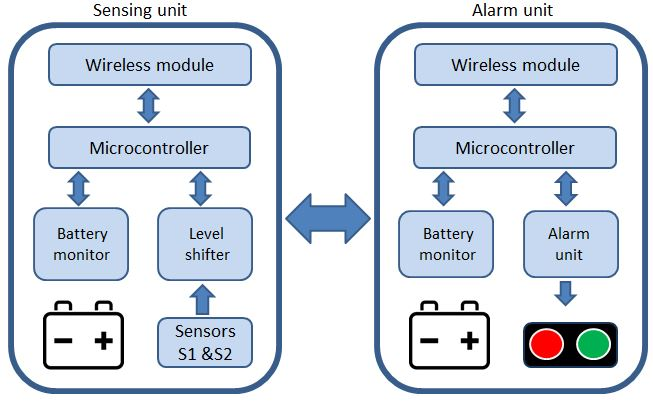
\includegraphics[height = 2.7in,width=4in,angle=00]{figures/sensorAlarm.JPG}
\caption{\small Hardware block diagram of the units}
\end{center}
\end{figure}
\newpage

These are the circuit diagrams of sensor unit and alarm unit:
\subsection{Sensor unit}
\mbox{} \\ \\
\begin{figure}[H]
\begin{center}
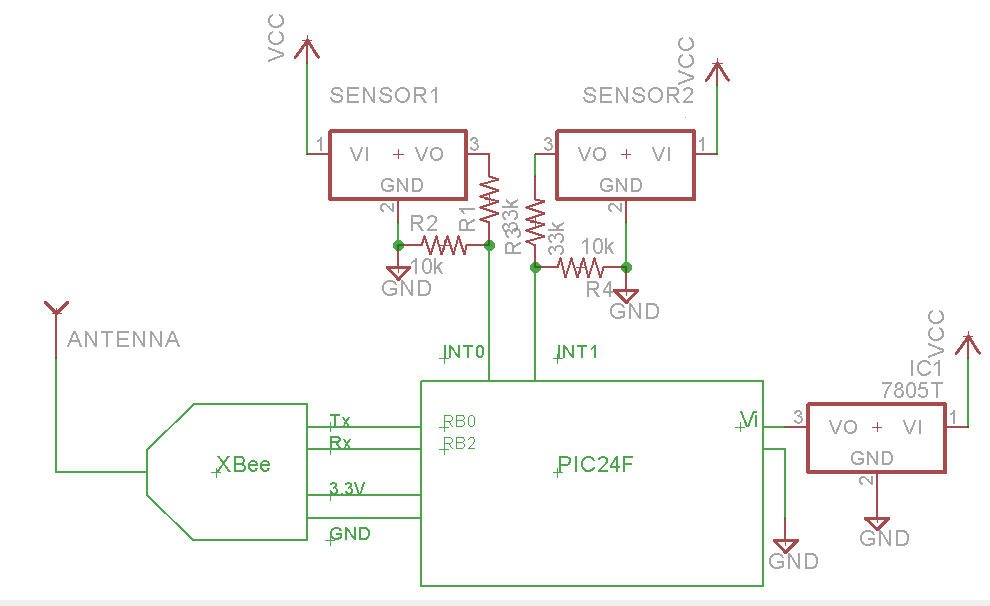
\includegraphics[height = 5in,width=7in,angle=00]{figures/sensorCircuit.png}
\caption{\small Sensor unit circuit diagram}
\end{center}
\end{figure}
The output of inductive proximity sensor when a metal is placed in its range is 12 V (Vcc). A voltage
divider, (R1, R2) in the circuit, is used to bring down this voltage to 3V, the input high voltage of
microcontroller. The system is powered by battery via a voltage regulator. XBee takes power from
microcontroller.\newpage
 \subsection{Alarm unit}
\mbox{} \\ \\ \\

\begin{figure}[H]
\begin{center}
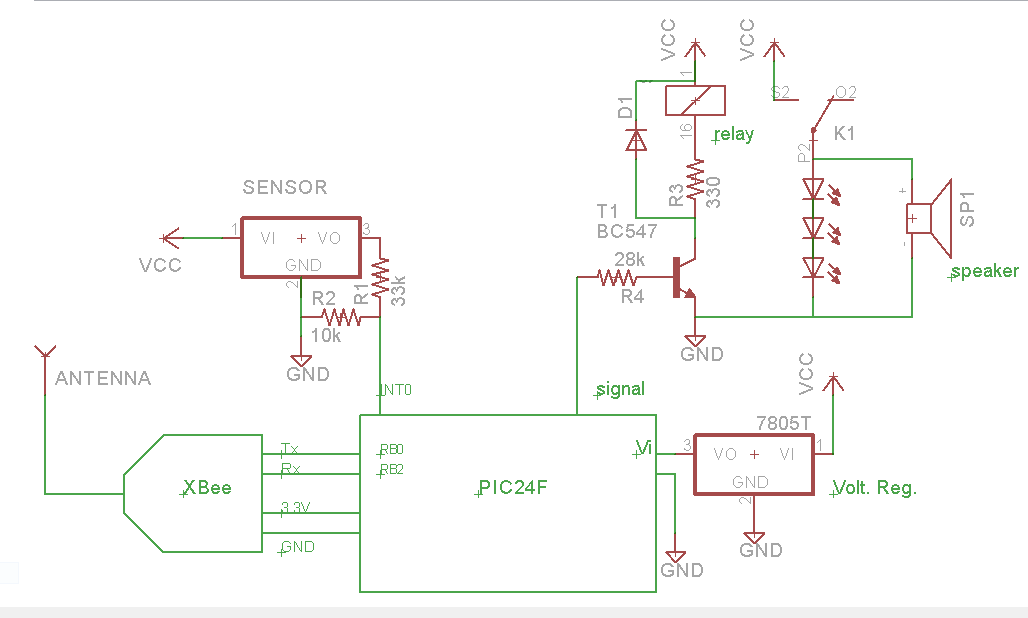
\includegraphics[height = 5in,width=7in,angle=00]{figures/alarmCircuit.png}
\caption{\small Alarm unit circuit diagram}
\end{center}
\end{figure}
When this unit receives train detected message from the sensor unit, the signal pin of microprocessor will
be made high. This turns on the transistor switch which draws 30mA of current via relay coil, enough to
turn on the relay switch which connects alarm (LEDs + speaker) and battery.


\newpage
\section{Photographs}
\mbox{}
\\
\begin{figure}[H]
\begin{center}
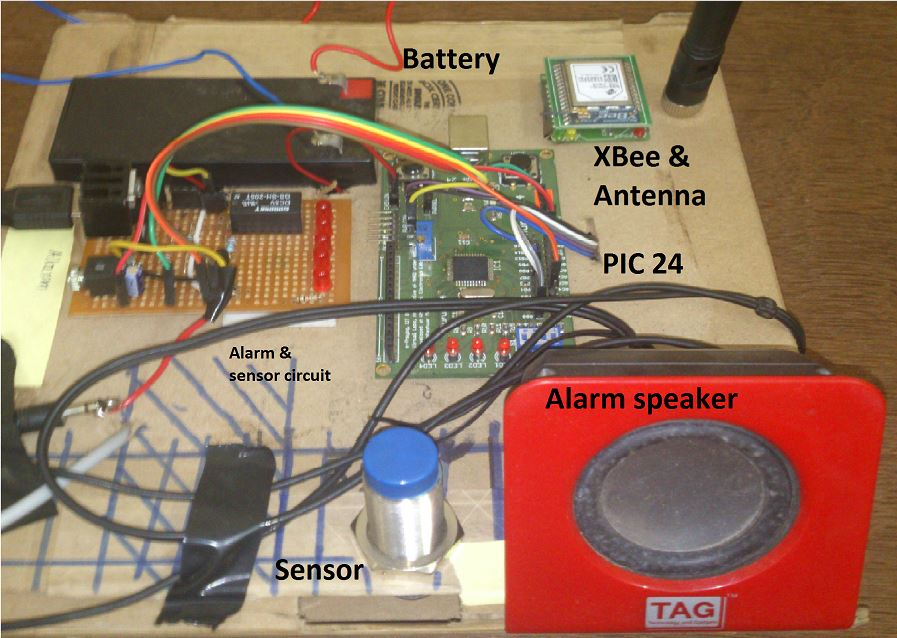
\includegraphics[height = 5in,width=7in,angle=00]{figures/alarmUnit.JPG}
\caption{\small Alarm Unit}
\end{center}
\end{figure}
\newpage
\mbox{}
\\ \\ \\
\begin{figure}[H]
\begin{center}
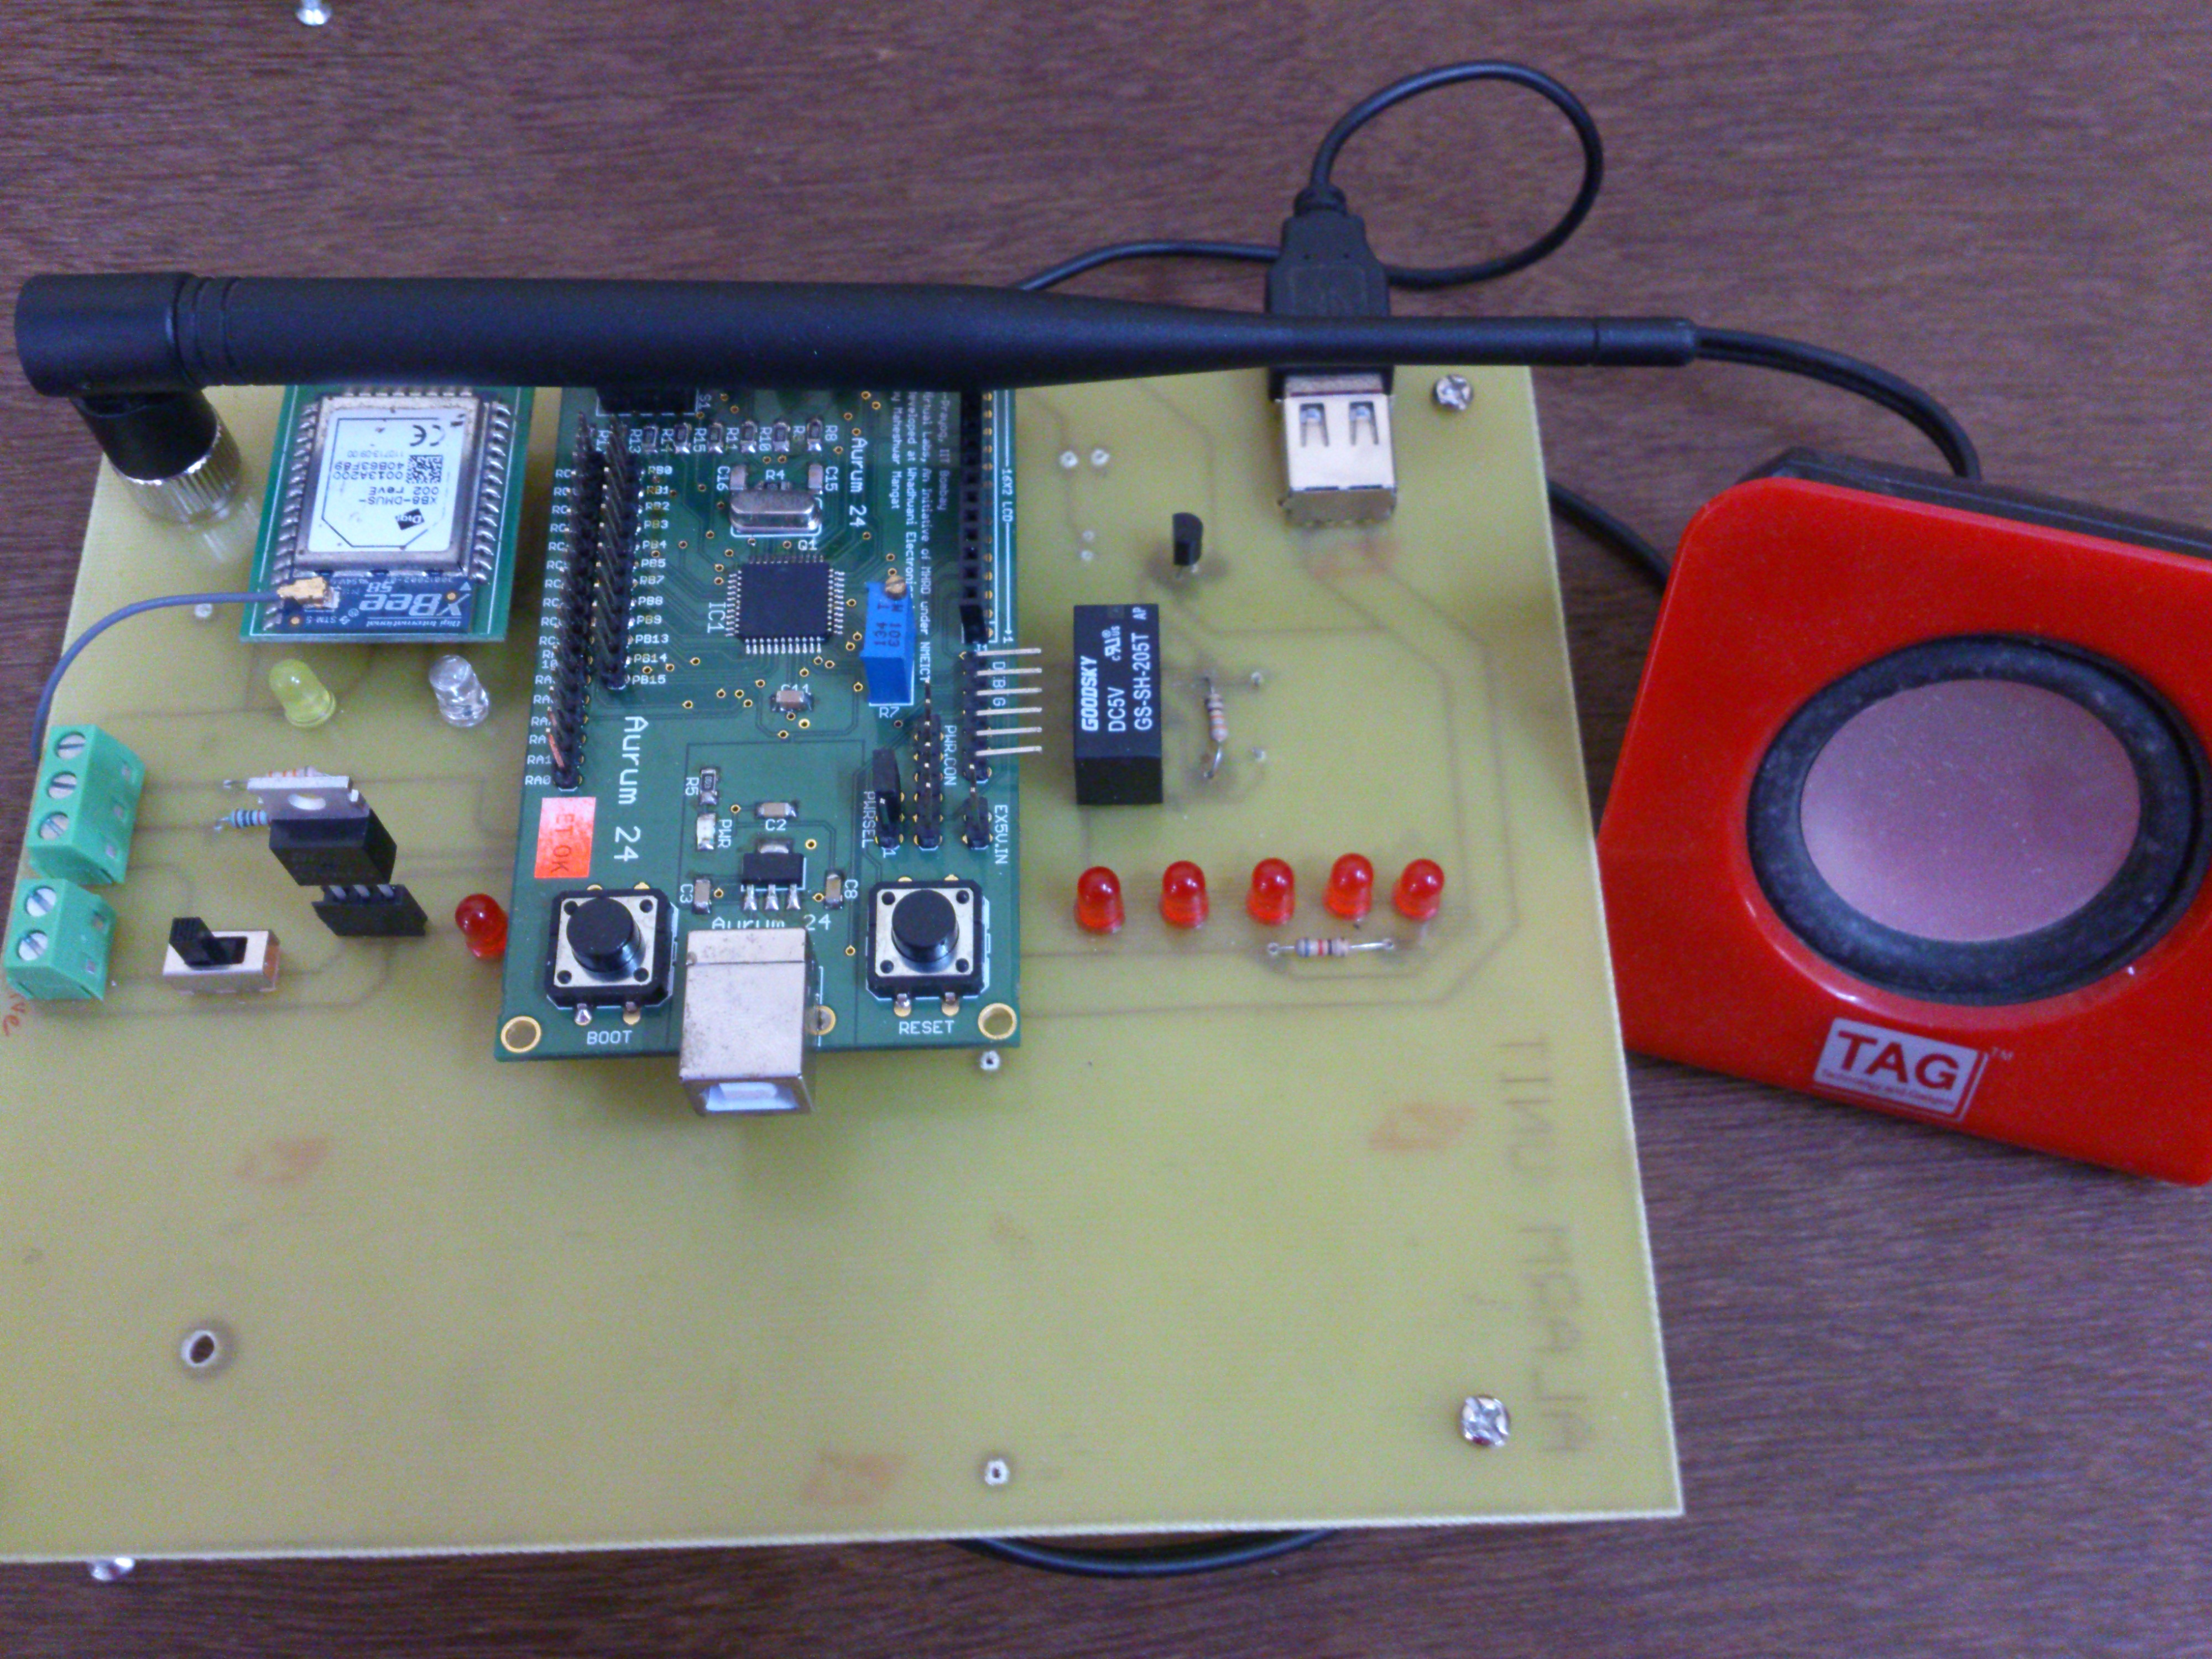
\includegraphics[height = 5in,width=7in,angle=00]{figures/alarmPCB.jpg}
\caption{\small PCB version of alarm unit}
\end{center}
\end{figure}
\newpage
\mbox{}
\\ \\ \\
\begin{figure}[H]
\begin{center}
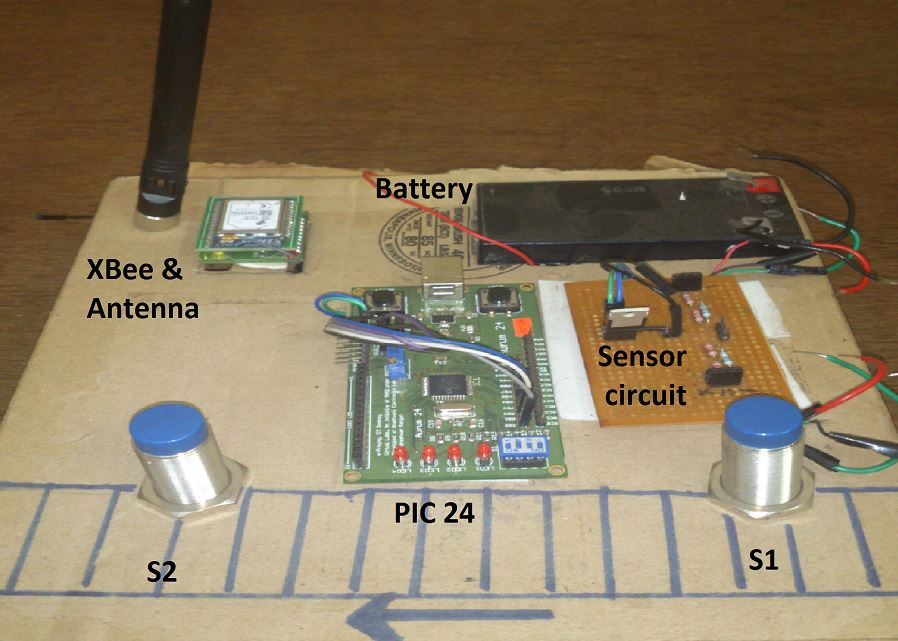
\includegraphics[height = 5in,width=7in,angle=00]{figures/sensorUnit.JPG}
\caption{\small Sensor Unit}
\end{center}
\end{figure}
\newpage
\mbox{}
\\ \\ \\
\begin{figure}[H]
\begin{center}
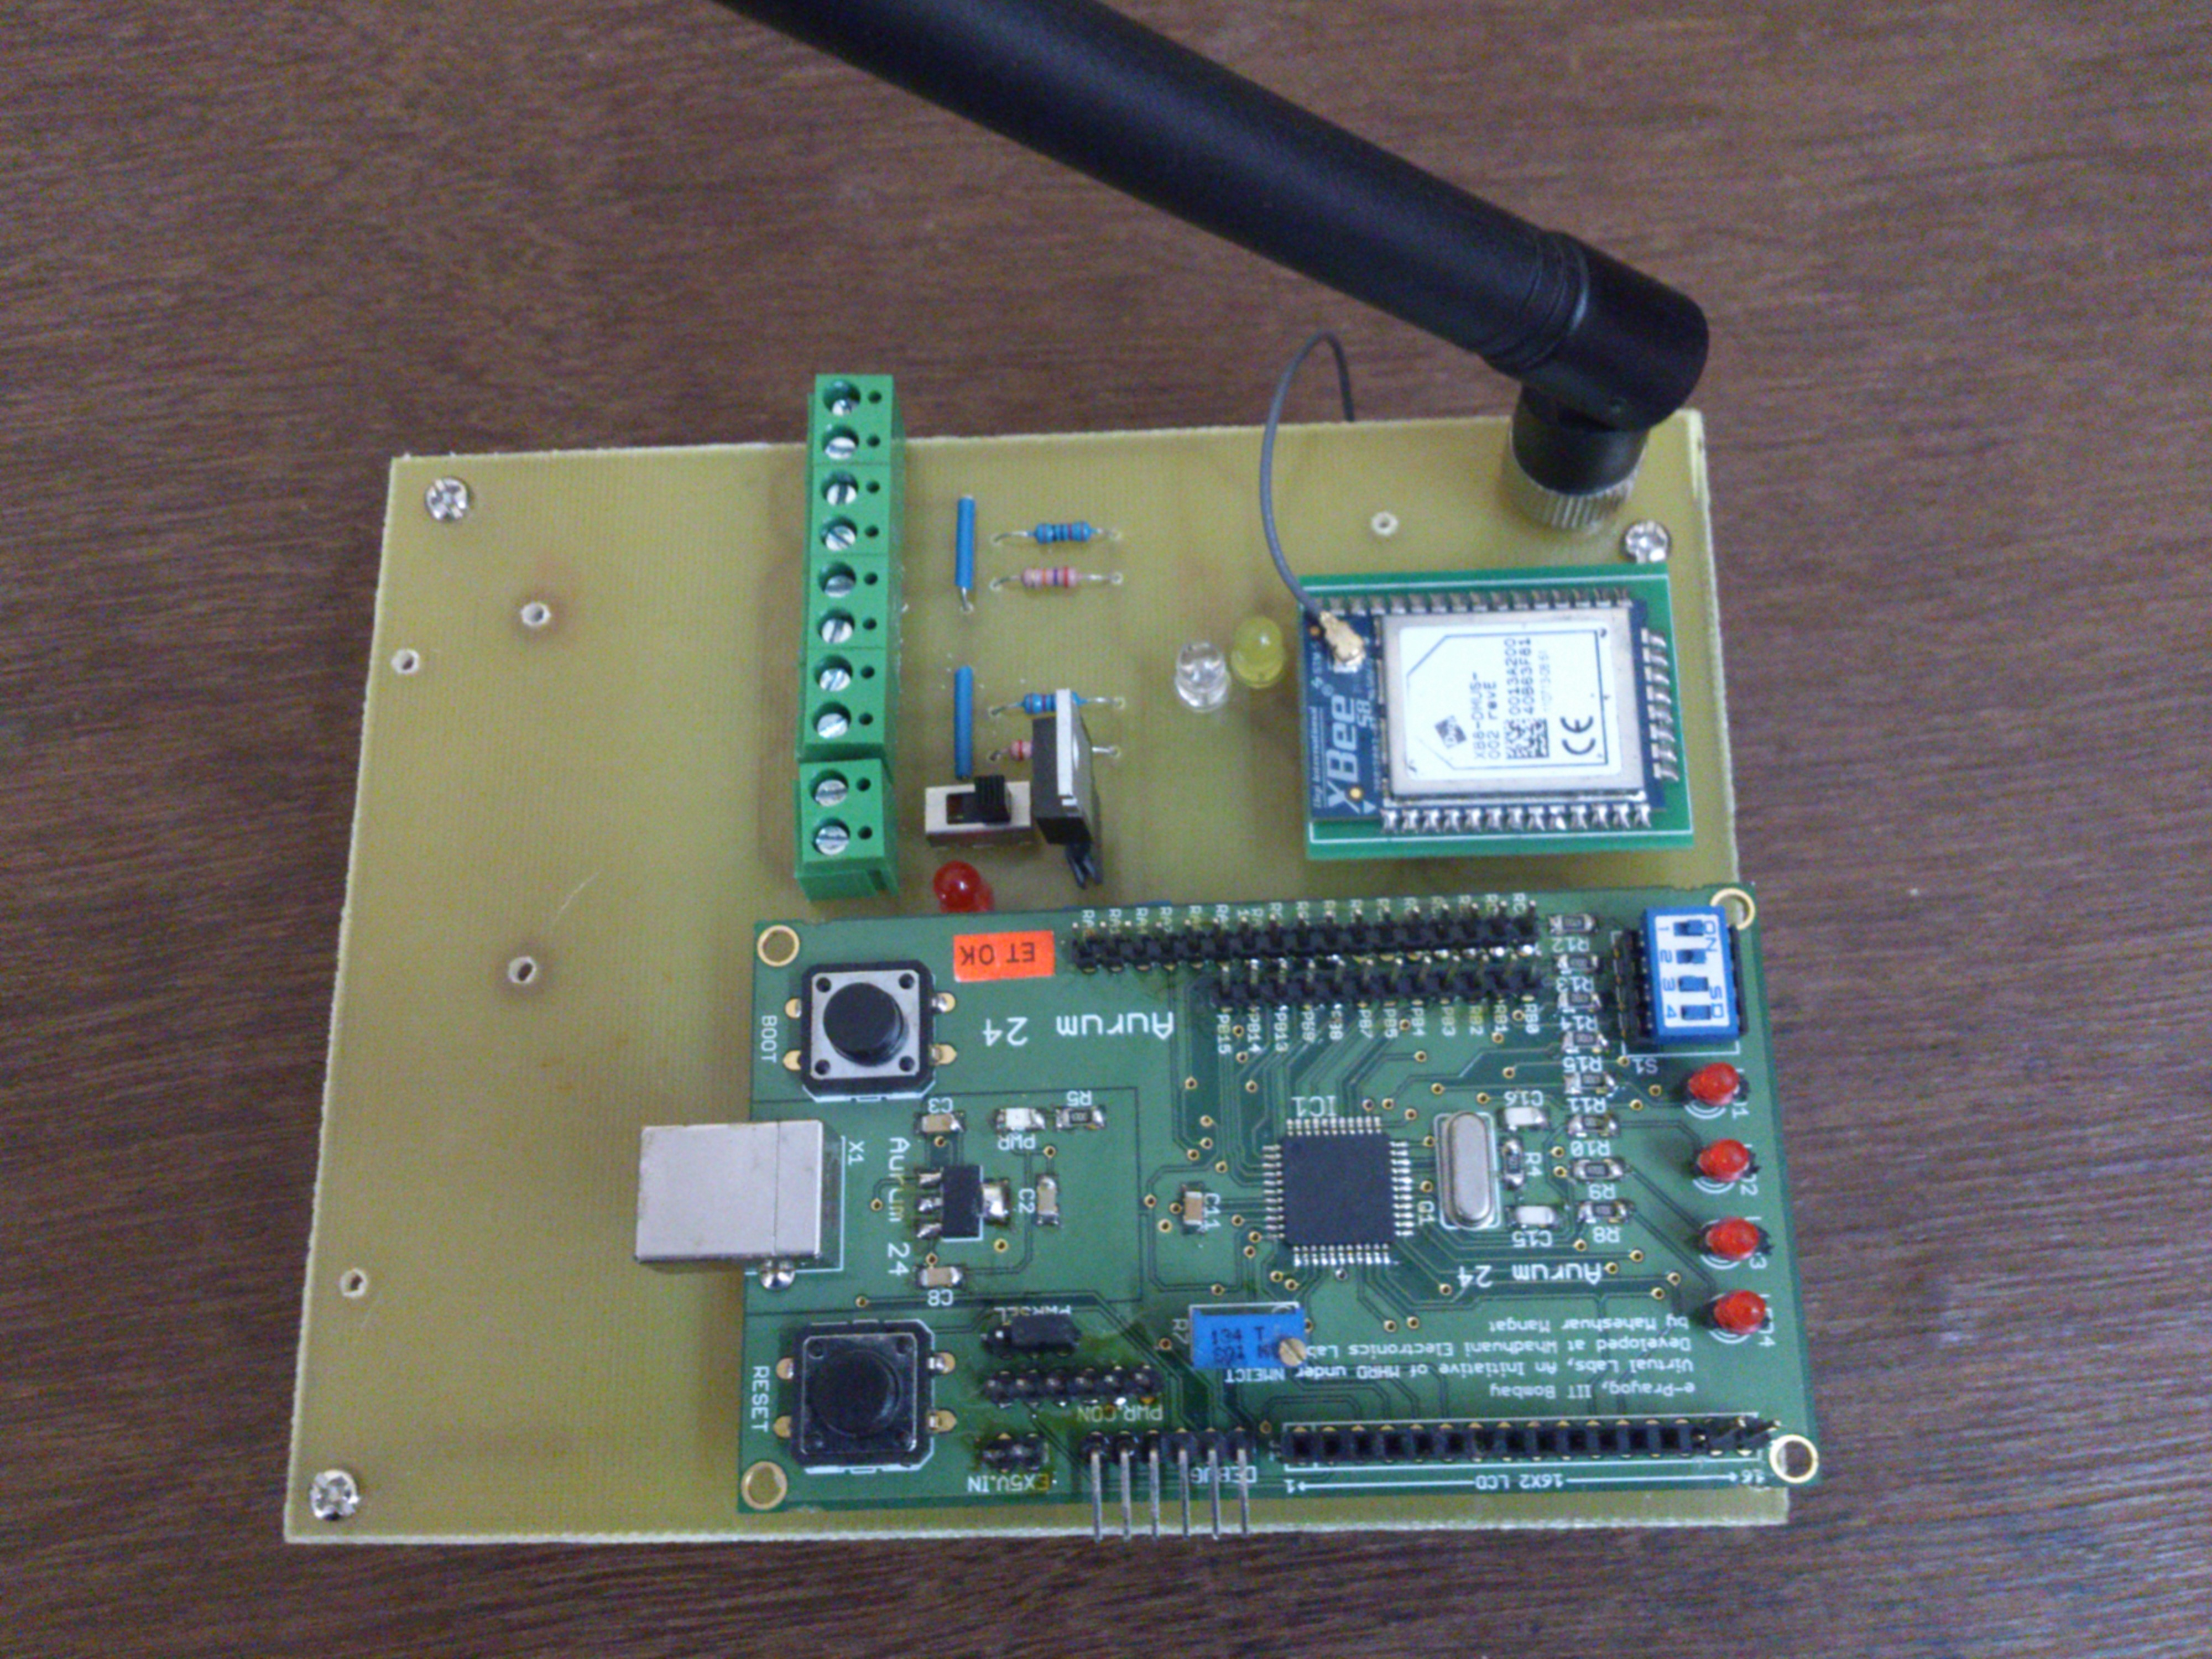
\includegraphics[height = 5in,width=7in,angle=00]{figures/sensorPCB.jpg}
\caption{\small PCB version of sensor unit}
\end{center}

\end{figure}
\begin{figure}[H]
\begin{center}
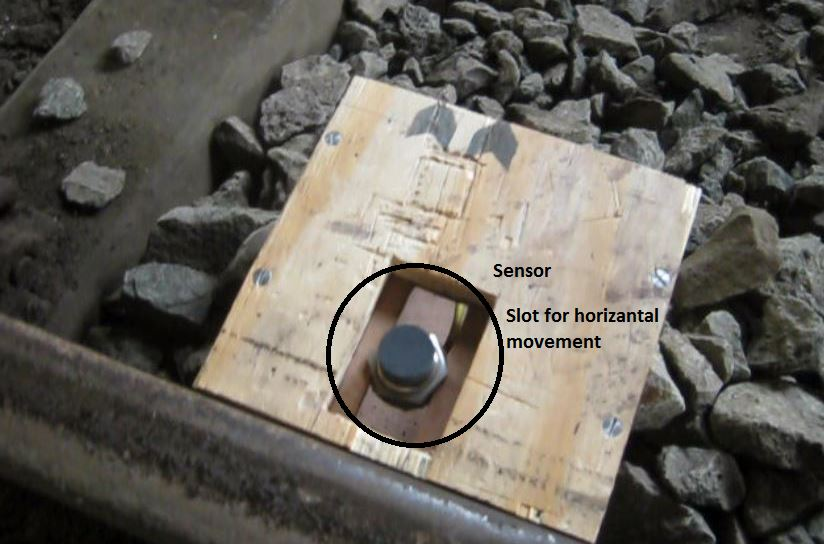
\includegraphics[height = 3in,width=4in,angle=00]{figures/sensor1.JPG}
\caption{\small Sensor arrangement at alarm unit}
\end{center}
\end{figure}

\section{Objectives achieved}
The algorithm to detect arrival of train on a unidirectional track has been implemented and tested by
giving manual pulses in lab. This was also tested on railway track with an 4-axle track machine in our
first field trip. \\ \\
The system was also tested by giving false/non-uniform pulses. Alarm turned on when the pulses were
given, but turned off the moment sensor unit detected that it was false alarm (the pulses were not similar
to those from a train). The system was working as expected in all cases. \\ \\
After testing the system for unidirectional, we moved on to modify the system to work in the case of
bidirectional track. The algorithm to detect the direction of the train was implemented and tested. \\
To test the system for bidirectional track, pulses were generated by using another microprocessor. The
system was tested on the track in our second trip. It detected the
direction but couldn't distinguish a false alarm and an accelerating machine i.
e. when the machine accelerated over the sensors, it gave a false alarm.
\\
\section{Problems faced}\
\textbf{UART on PIC24 :} \\
The first problem we faced was implementing UART. We need to write a value to the
UxBRG register to control baud rate. In the datasheet, the register value to get a baud rate of 9600 was
mentioned to be 25. But with that value, it was not working, we were getting random symbols. It was
debugged by coding the microprocessor to change the register value for each transmission and noting
down its value for correct transmission. It was later found out that the microcontroller board issued by the
lab has different crystal frequency than the one mentioned in the datasheet.
\\ \\
\textbf{Sensors arrangement on track:} \\
Sensors should be arranged on the tracks in such a way that the wheels of the train
should be at most 1 inch from the sensor for correct detection. We had to move the track machine to and
fro a couple of times to get the placement right. To solve this, proper measurements were taken and boxes
are being made so that anyone can place them correctly.
\\ \\
\textbf{Accelerating train :}
\\
The algorithm for finding out the direction of the train and the method to find if the
pulses are from sources other than a train have some correlation. When the track machine accelerated
over these sensors, the system gave a false alarm i.e. alarm turned on when the train was detected by
sensors unit but turned off before the track machine reached the alarm unit.
\section{Conclusions}
Judging by the fact that all the objectives listed at beginning of the project are achieved, the project is
complete. But the system was not tested extensively under all conditions and has no to check
working of all the devices in the system. A lot work has to be done to make it deployable.
\section{Future Work}
\begin{itemize}
  \item Designing a self-diagnosing system
  \item Checking the reliability by installing the system at a known location and logging all the data
  \item Designing standard directional antennas following power injection specifications
  \item Designing a new microcontroller by removing unnecessary parts in the present board
  \item Testing the system under different weather conditions
  \item Complete documentation of the project
\end{itemize}

\section{References}
\begin{itemize}
  \item \href{http://www.microchip.com.tw/Data_CD/Datasheet/16-Bits/39940C.pdf}{\textbf{PIC24FJ64GB004 family data sheet}}
  has everything related to the microprocessor but should be used keeping in mind that the system clock of the board might
  be different from that used for some calculations in the datasheet.
  \item The syntax to write ISRs and the lengths of various data types are listed
  in \href{http://ww1.microchip.com/downloads/en/devicedoc/c30_users_guide_51284f.pdf}{\textbf{MPLAB C30
  compiler user's guide}}
  \item For XBee module specs and documentation: \href{http://www.digi.com/products/wireless-wired-
  embedded-solutions/zigbee-rf-modules/zigbee-mesh-module/xbee-865lp}{\textbf{Digi website}}
\end{itemize}

\end{document}
